\documentclass{beamer}
\usepackage{tikz}
\usetikzlibrary{trees,arrows}
%\usepackage{subcaption}
\usepackage{csvsimple}

\usetheme{CMU}

\title{AutoMerge}
\subtitle{A Transportation Alternative for NYC}
\date{\today}
\author[Fonseca Mesner]{Francisco Fonseca \and Octavio Mesner}
\institute{Carnegie Mellon University}

\begin{document}
\maketitle

%\section{}
%\begin{frame}
%\frametitle{Goals}
%Discuss
%\begin{itemize}
%\item Outline Problem
%\item Alternatives
%\item Explain Costs and Calculations
%\item Specify Uncertainty
%\item State Assumptions
%\item Show Results
%\item Convey Sensitivity Analyses
%\item Conclusion
%\end{itemize}
%\end{frame}

\section{Problem}

\begin{frame}
  \frametitle{Problem}
  \begin{block}{Overview}
  \begin{itemize}
  \item NYC plans to become a leader in \emph{smart city} infrastructure
  \item One piece: Evaluate autonomous vehicles
  \item By 2020, NYC expects its fleet to be autonomous.
  \item We will evaluate AutoMerge (AM) Inc as an alternative.
  \end{itemize}
  \end{block}
\end{frame}

\section{Alternatives}
\begin{frame}
  \frametitle{Alternatives}
  \begin{block}{Description}
  \begin{description}
  \item[Alternative 1] Do Not Implement AM.\\
    This are the costs that would be incurred if the status quo
    continues so there is little uncertainty for this alternative.
  \item[Alternative 2] Implement AM.\\
    Implementing AM comes with uncertainty with respect to AM
    performance.
  \item [Alternative 3] Perform a pilot study.\\
    We decide size of pilot study.  A larger the study reduces more
    uncertainty than a smaller one but costs more.
  \end{description}
  \end{block}
\end{frame}

\section{Costs}
\begin{frame}
  \frametitle{Some Costs,  Calculations, and Assumptions}
  \begin{block}{Congestions, Capital, and Human costs}
    \begin{table}[h]
      % \caption{Capital and O\&M costs of the AM system}
      \centering
      \tiny
      %\renewcommand{\arraystretch}{1.1}
      \begin{tabular}{c l l l}
        \hline
 	& Variable & Value & Notes \\\hline\hline
        (a)& \# buses with age $<$ 5 years& 2313& Source: \cite{am1}\\
(b)	& \# buses with age 5-9 years				& 1296				& Source:	\cite{am1}					\\
(c)	& \# buses with age 10-20 years			& 1437				& Source:	\cite{am1}					\\
(d)	& Capital Cost per bus age $<$ 5 years		& \$ 5000				& Source:	\cite{am1}		\\
(e)	& Capital Cost per bus age 5-9 years		& \$ 6500				& Source:	\cite{am1}		\\
(f)	& Capital Cost per bus age 10-20 years		& \$ 8500				& Source:	\cite{am1}		\\
\textbf{(g)}	& \textbf{Total Capital Cost}(*)			& \textbf{\$ 45.7 Million}	& \textbf{=(a)*(d)+(b)*(e)+(c)*(f)}			\\
(h)	& Annual O\&M Cost per Bus				& \$ 1500				& Source:	\cite{am1}	\\
\textbf{(i)}	& \textbf{Total Annual O\&M Cost} (**)	& \textbf{\$
  7.6 Million}	& \textbf{=[(a)+(b)+(c)]*(h)}\\
(j)	& Annual Cost per Commuter				& \$ 1739				& Source:	\cite{UMR}	\\
(k)	& Annual hours in congestion per commuter	& 74 hours			& Source:	\cite{UMR} 	\\
(l)	& Cost per minute 						& \$ 0.39				& $(h)/[(i)*60]$		\\
(m)	& Total person trip per day					& 1.52 million			& Source: 	\cite{nyctransit}	\\
(n)	& Average time in daily person trip			& 49 minutes			& Source:	\cite{nyctransit}	\\
\textbf{(o)}	& \textbf{Total annual congestion cost}	& \textbf{\$
  10.5 Billion}	& \textbf{=360*l*(k)*(j)}\\
(p)	& VSL (2015 \$)						& \$ 8.7 Million			& Source:	\cite{EIA:guidelines}		\\
(q)	& Number of fatalities per year				& 16					& Source: \cite{nyctransit}	\\
\textbf{(r)}	& \textbf{Total annual mortality cost}	& \textbf{\$ 150 Million}	& \textbf{=(p)*(q)}			\\
(s)	& Average Cost of Injury 					& \$ 179,000			& Source:	\cite{CDC} 	\\
(t)	& Number of injuries per year				& 1740				& Source:	\cite{nyctransit}	\\
\textbf{(u)}	& \textbf{Total annual injury cost}	& \textbf{\$ 311 Million}		& \textbf{=(s)*(t)}
\\\hline\hline
%\multicolumn{4}{l}{{\footnotesize (*) Capital costs are considered to be incurred only in the first year}} \\
%\multicolumn{4}{l}{{\footnotesize (**) O\&M costs begin to occur in the fifth year of the analysis (when AM starts operating)}} \\
\end{tabular}
%\label{tab:am.cost}
\end{table}%
\end{block}
\end{frame}

\section{Uncertainty}
\begin{frame}
  \frametitle{Uncertainty}
  \begin{columns}
    \begin{column}{0.7\textwidth}
      \centering
      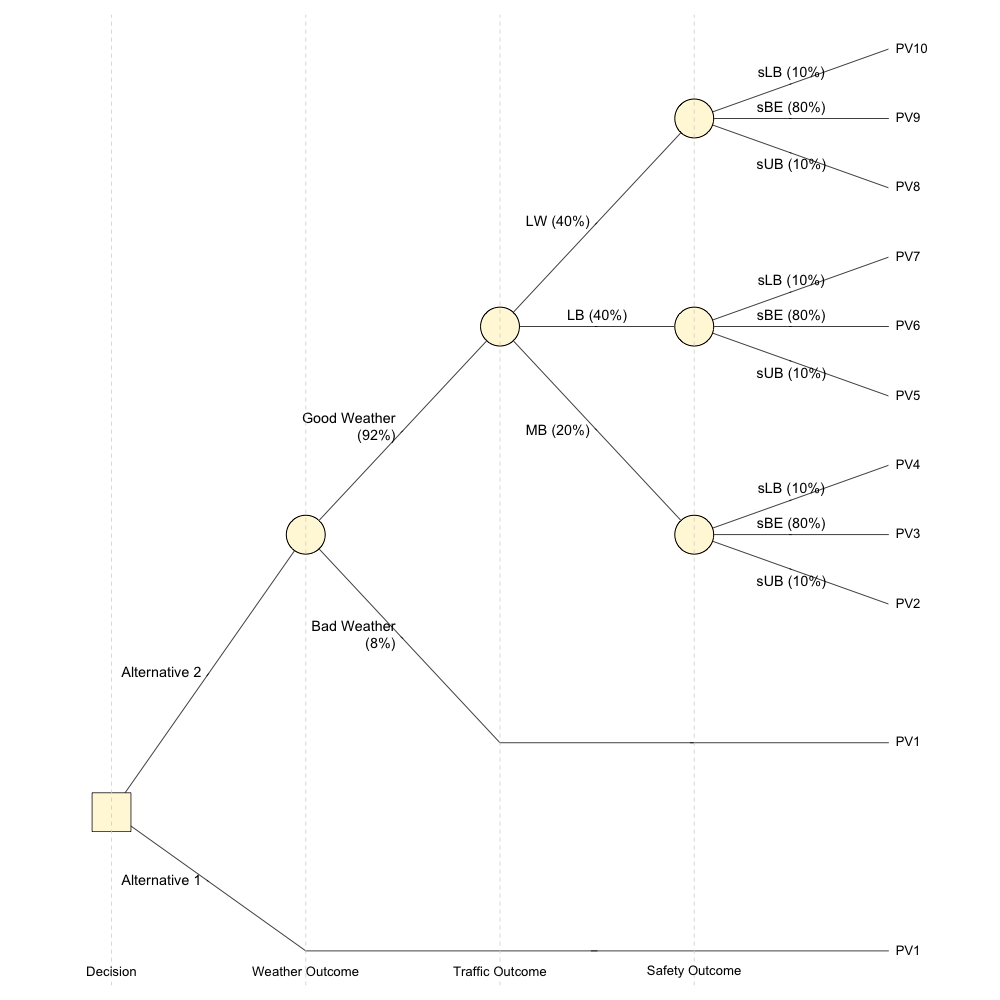
\includegraphics[width=\textwidth]{../../R/decisiontree}
    \end{column}
    \begin{column}{0.4\textwidth}
      \begin{itemize}\small
      \item We account for uncertainty using decision trees.
      \item Source of uncertainty: Performance, Safety, and Weather
      \item We calculated Expected NPV for each outcome to evaluate.
      \end{itemize}
    \end{column}
  \end{columns}
\end{frame}

\section{Results}
\begin{frame}
  \frametitle{Results}
      \begin{itemize}
        \item Alternative 2 outperforms 1 in total cost.
        \item Congestion costs are based on total travel time.
      \end{itemize}
    \begin{block}{Expected Cost in Billions (\$)}
      \centering \footnotesize
      \begin{tabular}{l c c}
        \hline
        & Alternative 1 & Alternative 2\\
        \hline\hline
        Capital Costs & 0 & 0.05\\
        O\&M & 0 & 0.06\\
        Mortality & 1.45 & 1.39\\
        Injury & 3.23 & 3.11\\
        Congestion* & 109.12 & 107.16\\
        Air Pollution & 10.55 & 10.55\\
        GHG & 0.8 & 0.8\\
        \hline
        Total & 125.15 & 123.12\\
        \hline\hline
      \end{tabular}
    \end{block}
\end{frame}


\section{Pilot Study}
\begin{frame}
  \frametitle{Pilot}
  \begin{columns}
    \begin{column}{0.4\textwidth}
      \begin{itemize}
      \item Uses EVII and Bayes Theorem to compute
      \item Figure shows value study after associated cost.
      \item Value optimized at 100\% of fleet
      \end{itemize}
    \end{column}
    \begin{column}{0.6\textwidth}
      \centering
      \includegraphics[width=\textwidth]{../../R/alt3barplot}
    \end{column}
  \end{columns}
\end{frame}

\section{Sensitivity}
\begin{frame}
  \frametitle{Sensitivity Analyses}
  \begin{columns}
    \begin{column}{0.4\textwidth}
      \begin{itemize}
      \item Input values varied between 50 and 200\% or more.
      %\item Dashed line indicates baseline assumption
      \item Discount rate, VSL, and per person cost of commute time
        all greatly affect net expected cost but similarly for all.
      \item Weather affects alternatives 2 and 3 more then 1 but
        alternative 1 remained more expensive.
      \end{itemize}
    \end{column}
    \begin{column}{0.65\textwidth}
      \centering
      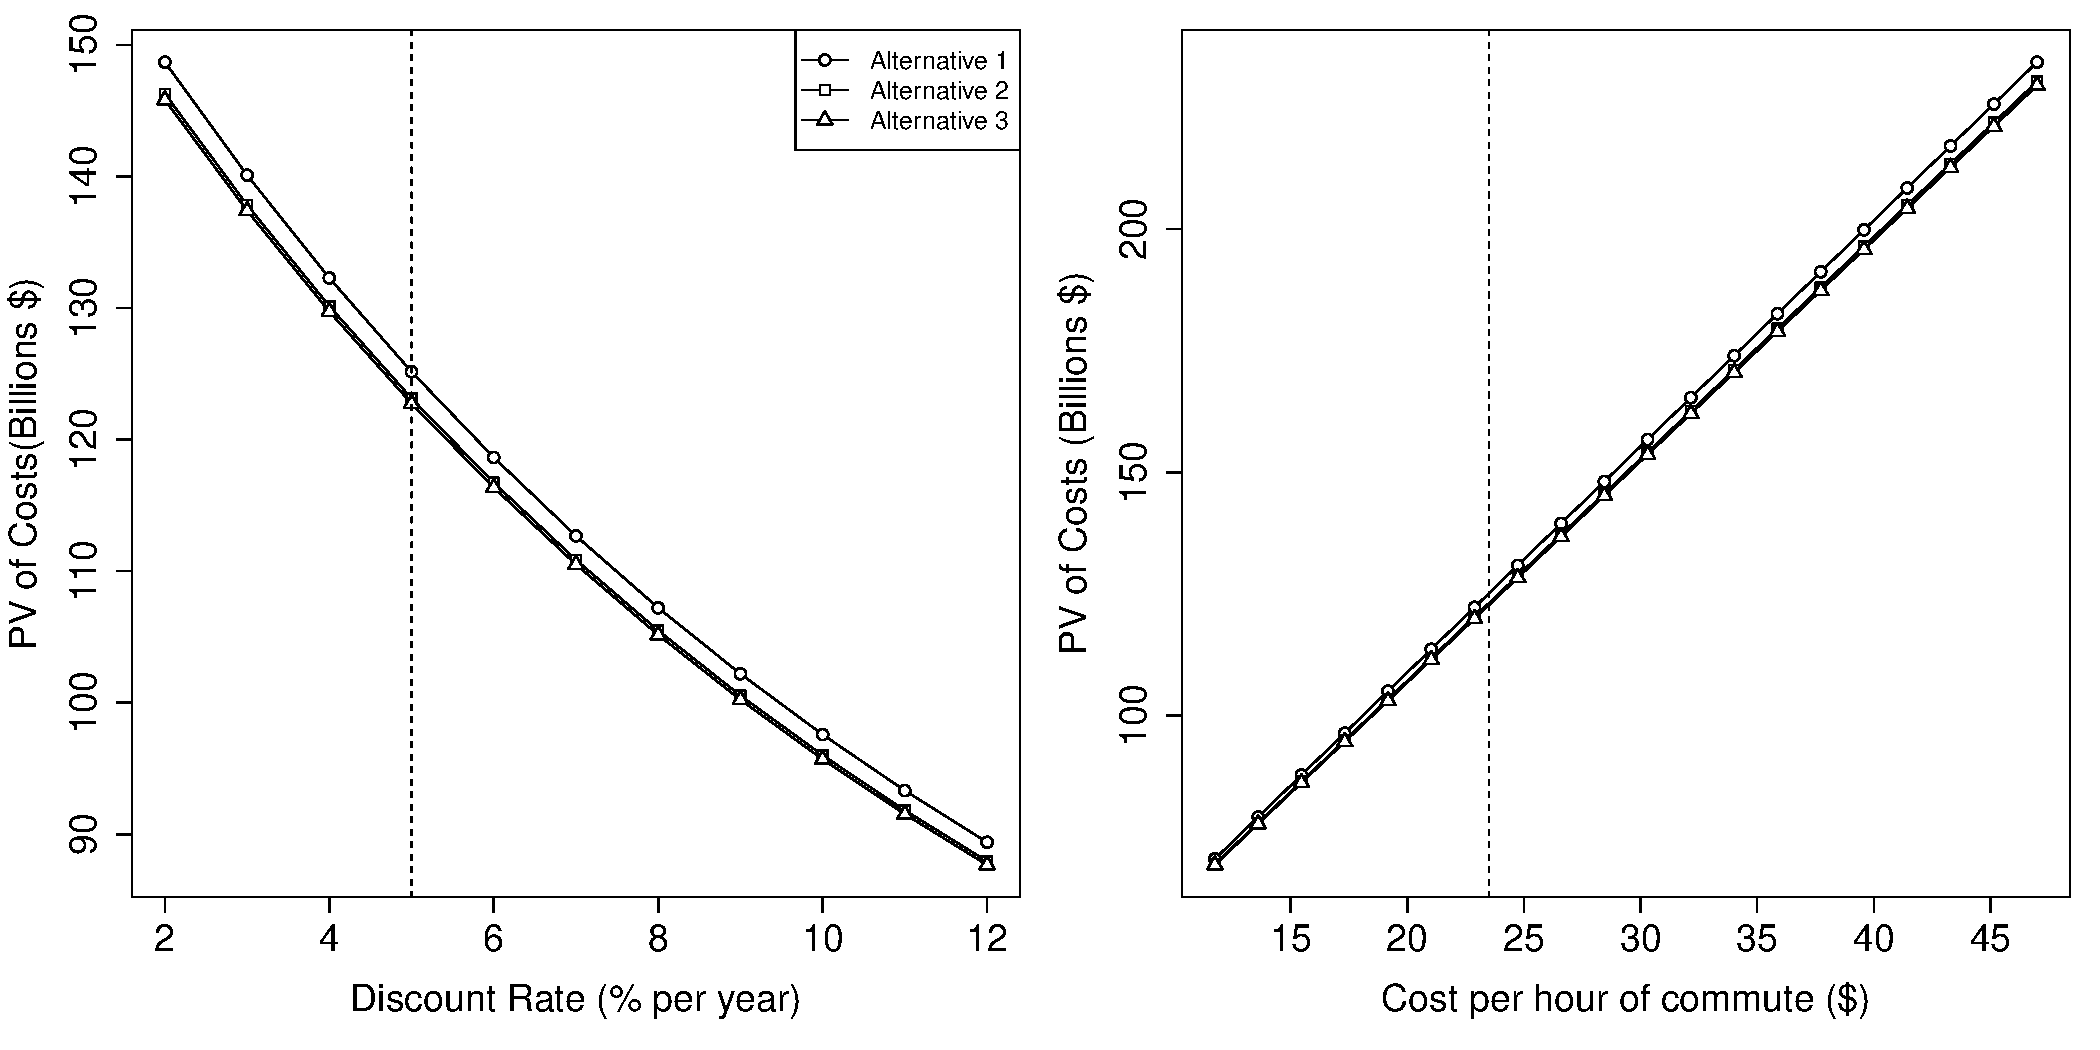
\includegraphics[width=.9\textwidth]{../../R/sensitivity1}\\
      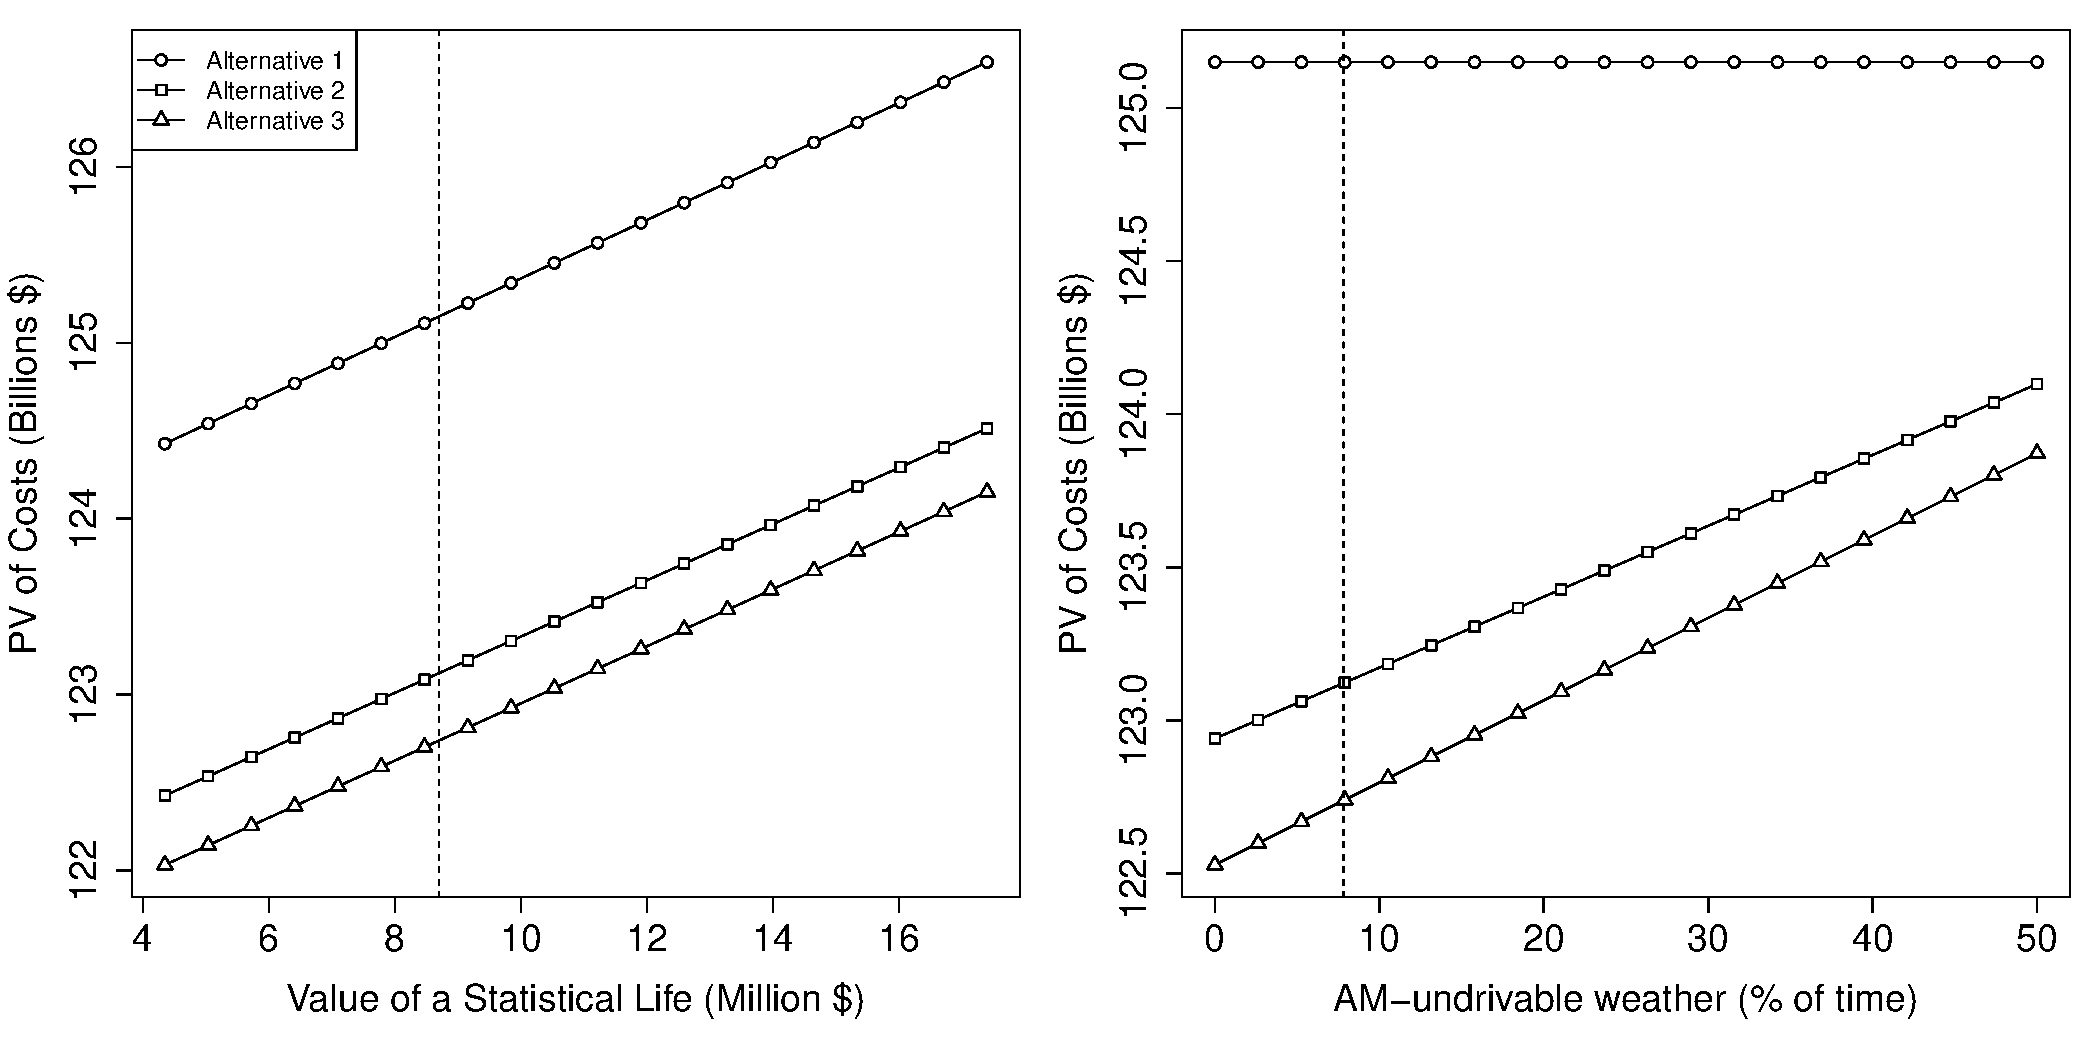
\includegraphics[width=.9\textwidth]{../../R/sensitivity2}
    \end{column}
  \end{columns}
\end{frame}

\section{Conclusion}
\begin{frame}
  \frametitle{Conclusion}
  \begin{itemize}
  \item Given uncertainty, investing in AM reduces cost over not investing.
  \item Using a risk-neutral metric, performing any pilot study with
    at least 50\% of fleet adds value.
  \item Using 100\% of fleet maximized value
  \item This recommendation is robust to necessary assumptions.
  \end{itemize}
\end{frame}


\section{References}
\begin{frame}
  \frametitle{References}
  Questions? \\~\\
  \bibliography{../report/bibfile.bib}{}
  \bibliographystyle{amsalpha}
\end{frame}

\end{document}
